\documentclass{article}
%------------------------------------------------------------------------------
%\usepackage{embedall}
\usepackage[a4paper]{geometry}
\usepackage[utf8]{inputenc}
\usepackage[english]{babel}
\usepackage[numbered,framed]{mcode}
\usepackage{amsthm, amsmath, amssymb, gensymb, physics, upgreek, siunitx}
\usepackage{graphicx, epstopdf, float, hyperref, cleveref}
\usepackage[caption=false]{subfig}
\usepackage[version=4]{mhchem}
\usepackage{enumitem,verbatim}
\usepackage{matlabmatrix}
\usepackage{tikz} 

\usepackage[ruled,vlined]{algorithm2e}

\graphicspath{{../}}
\epstopdfsetup{outdir=./}

% Numbered environment
\newcounter{example}[section]
\newenvironment{example}[1][]{\refstepcounter{example}\par\medskip
	\textbf{Example~\theexample. #1} \rmfamily}{\medskip}

% Classic symbols
\newcommand{\me}{\mathrm{e}}
\DeclareMathOperator{\sgn}{sgn}
\DeclareMathOperator{\sinc}{sinc}
\newcommand{\bigo}[1]{\mathcal{O}\left(#1\right)}

% Set theory
\newcommand{\reals}{\mathbb{R}}
\newcommand{\integers}{\mathbb{Z}}

% Vector notation
\renewcommand{\vec}[1]{\mathbf{#1}}
\newcommand{\uvec}[1]{\mathbf{\hat{#1}}}
\newcommand{\transp}{\text{T}}
\newcommand{\adj}[1]{#1^\dagger}
\DeclareMathOperator{\diag}{diag}

\newcommand{\conj}[1]{{\overline{#1}}}
\newcommand{\imag}[1]{{\Im\left\{#1\right\}}}
\renewcommand{\real}[1]{{\Re\left\{#1\right\}}}
%------------------------------------------------------------------------------

\begin{document}

\newtheorem{theorem}{Theorem}
\makeatletter
\title{Lightning Stokes Solver}
\author{Pablo Brubeck \and Nick Trefethen}
\date{\today}
\makeatother

\maketitle

\begin{abstract}
Gopal and Trefethen have recently introduced ``lightning solvers''
for the 2D Laplace and Helmholtz equations, based on rational
functions with poles exponentially clustered near singular corners.
Making use of the Goursat representation in terms of analytic
functions, we extend these methods to the biharmonic equation,
specifically to 2D Stokes flow.  Flows in bounded, unbounded, and
multiply connected domains are considered, with solutions computed
to ten digits of accuracy in a few seconds of laptop time.  As an
illustration of the high accuracy, we readily resolve two or three
counter-rotating Moffatt eddies near a singular corner.
\end{abstract}

\linespread{1}

%------------------------------------------------------------------------------
\section{Introduction}
%------------------------------------------------------------------------------

In this paper we consider numerical solutions to the biharmonic equation in a
two-dimensional domain $\Omega\subseteq\reals^2$,
\begin{equation} \label{eq:bih}
\nabla^4 \psi = \nabla^2 \left(\nabla^2 \psi\right) 
   = \psi_{xxxx} +2\psi_{xxyy} +\psi_{yyyy} = 0,
\end{equation}
coupled with appropriate boundary conditions. Since the equation is of fourth
order, to ensure well-posedness, we impose two boundary conditions at each
point of $\partial\Omega$. We specify the value of the function itself and one
component of the gradient on a portion $\Gamma_1$ of $\partial\Omega$, and both
components of the gradient on the complementary part $\Gamma_2$,
\begin{subequations}\label{eq:bcs}
\begin{equation}
\psi = h(x,y), \quad \uvec{a}\cdot \nabla\psi = k(x,y)\quad \text{on }\Gamma_1,\\
\end{equation}
\begin{equation}
\nabla \psi = \vec{g}(x,y) \quad\text{on }\Gamma_2,
\end{equation}
\end{subequations}
where $\uvec{a}\in\reals^2$ is a fixed unit vector, with $\partial\Omega =
\Gamma_1 \cup \Gamma_2$ and $\Gamma_1\cap\Gamma_2 = \emptyset$. Functions that
satisfy \eqref{eq:bih} are called biharmonic and are smooth in the interior of
$\Omega$, although point-singularities may arise on the boundary when
$\partial\Omega$ contains corners or when the boundary data $h$, $k$, $\vec{g}$
have singularities, or at points of juncture between $\Gamma_1$ and $\Gamma_2$.

In this paper, we propose a numerical method to solve
\eqref{eq:bih}--\eqref{eq:bcs} by generalizing the recently introduced
``lightning solvers'' for the 2D Laplace and Helmholtz equations
\cite{gopal19,gopal19new}. The main advantage of this class of methods is that
they can handle very general singularities in very general domains with
corners, without requiring any detailed analysis, and still achieve high
accuracy.

This work is structured as follows. In Section \ref{sec:goursat}, we describe
the Goursat representation, which allows one to write any solution to
\eqref{eq:bih} in terms of two analytic functions when $\Omega$ is simply
connected. These two functions can then be approximated by rational functions
\cite{newman64}.  The biharmonic equation is most commonly found in
applications in Stokes flow and linear elasticity. In Section
\ref{sec:physics}, we review how the incompressible Stokes equations can be
represented via the stream function, which is biharmonic. For linear elasticity
problems, one transforms the governing equations into a biharmonic equation
involving the Airy stress function, but problems of elasticity are not explored
in this paper.

Our method consists of approximating both Goursat functions by rational
functions and finding coefficients that best satisfy the boundary conditions
\eqref{eq:bcs} in the least-squares sense. A detailed description of the
method, along with implementation details, is given in Section
\ref{sec:method}, and numerical results are presented in Section
\ref{sec:results}. The method gets high accuracy for simple geometries with
great speed, and we illustrate this by showing its ability to easily resolve
two or more Moffatt eddies in corners. In Section \ref{sec:unbounded}, we show
how to extend the method to unbounded domains directly without the need for
artificial boundaries. Section  \ref{sec:multiply} presents an extension to
multiply connected regions by the inclusion of additional logarithmic terms.
Finally, we give our conclusions in Section \ref{sec:conclusion}.

%------------------------------------------------------------------------------
\section{Biharmonic functions in simply-connected domains \label{sec:goursat}}
%------------------------------------------------------------------------------

The Goursat representation is the key ingredient required to extend the
lightning solver to biharmonic problems, going back to the French mathematician
Goursat in 1898 \cite{goursat98}. It allows one to represent biharmonic
functions in terms of two analytic functions, which our algorithms will then
approximate by rational functions. In line with the use of analytichttp
functions, and throughout the rest of the paper, we represent $x$ and $y$ via
the complex variable $z = x + iy$. We include a precise statement of the
Goursat representation in the form of a theorem, along with two proofs, which
we consider to be valuable in giving two perspectives on what is going on. The
original proof was given by Goursat in \cite{goursat98}, and an alternative
proof is given by Muskhelishvili in \cite{musk19}. Both of these are also found
in textbooks such as \cite{carrier05,musk77}. Although we label them
``proofs'', we don’t give these arguments in full detail. For a rigorous
discussion, see \cite{musk77}.


\begin{theorem}[Goursat representation]
\label{th:goursat}
Let $\Omega\subseteq\mathbb{C}$ be a simply-connected open region, and let
$\psi : \Omega \to \reals$ be a biharmonic function. Then $\psi$ can
be represented in terms of functions $f(z)$ and $g(z)$ analytic in $\Omega$
by the formula
\begin{equation}\label{eq:goursat}
\psi(x,y) = \psi(z,\conj{z}) = \Im \left\{ \conj{z}f(z) + g(z)\right\}.
\end{equation}
The functions $f(z)$ and $g(z)$ are uniquely defined up to addition of
arbitrary terms $\lambda z+C$ to $f(z)$ and $\conj{C}z+\alpha$ to $g(z)$,
where $\lambda,\alpha\in\reals$ and $C\in\mathbb{C}$.
\end{theorem}

The use of the imaginary as opposed to the real part is standard in the
literature and helps to simplify the expressions for physical quantities
associated with $\psi$. Series expansions based on \eqref{eq:goursat} have been
used to find numerical solutions to BVPs associated with \eqref{eq:bih} by
Gaskell et al. in \cite{gaskell98}, Finn, Cox and Byrne in \cite{finn03}, and
by Luca and Crowdy in \cite{luca18}, among many others. Though the Goursat
representation has been used by various people over the years, it is used far
less than more general tools such as FEM and integral equations and indeed is
surprisingly hard to find in textbooks.

\begin{proof}[Goursat's proof \cite{goursat98}]
First, we note that the biharmonic operator can be written in terms of
Wirtinger derivatives,
\begin{equation}
\nabla^4 \psi = 16\frac{\partial^4 \psi}{\partial\conj{z}^2 \partial z^2}.
\end{equation}
Treating $z$ and $\conj{z}$ as independent variables, one can solve this
equation by separation of variables. Under the assumption that $\psi$ is
analytic with respect to the real variables $x$ and $y$, we may plug in the
ansatz $\psi=\sum_k \psi_k$, where $\psi_k= A_k(z)B_k(\conj{z})$, obtaining
\begin{equation}
\frac{\partial^4 \psi_k}{\partial\conj{z}^2 \partial z^2} 
   = A_k''(z) B_k''(\conj{z}) = 0,
\end{equation} 
which implies that either $A_k''(z)=0$ or $B_k''(\conj{z})=0$. The solution
spaces for these two cases are spanned by $\{1,z\}$ for $A_k''(z)=0$  and
$\{1,\conj{z}\}$ for $B_k''(\conj{z})=0$. Therefore, without loss of
generality, by superposition of the four independent solutions,
\begin{equation}
\psi(z,\conj{z}) =  A_1(z) + \conj{z} A_2(z) + B_3(\conj{z}) + z B_4(\conj{z}),
\end{equation}
where $A_1(z), A_2(z), B_3(\conj{z}), B_4(\conj{z})$ are arbitrary functions.
Since $\psi$ must be real, $\psi=\conj{\psi}$ implies that 
\begin{equation}
\psi(z,\conj{z}) =  A_1(z)  + \conj{z} A_2(z)  + \conj{A_1(z)} + z \conj{A_2(z)} 
                 = 2 \Re\left\{A_1(z) + \conj{z} A_2(z)\right\},
\end{equation}
which implies \eqref{eq:goursat} by letting $f(z) = -2i A_2(z)$
and $g(z) = -2i A_1(z)$. We finally note that, when $\psi$ is given, $f(z)$
and $g(z)$ are determined up to an additive linear term. To be more precise,
the substitutions $f(z)\to f(z)+\lambda z + C$ together with $g(z)\to
g(z)+\conj{C}z+\alpha$ for $\lambda,\alpha\in\reals$ and $C\in\mathbb{C}$
leave $\psi$ invariant.
\end{proof}

\begin{proof}[Muskhelishvili's proof \cite{musk19}]
If $\omega=-\nabla^2 \psi$, then $-\nabla^2\omega = \nabla^4\psi = 0$. Now
define $p$ as the harmonic conjugate of $\omega$, satisfying the
Cauchy-Riemann conditions
\begin{equation}
\frac{\partial\omega}{\partial x} = \frac{\partial p}{\partial y}, \quad
\frac{\partial\omega}{\partial y} = -\frac{\partial p}{\partial x};
\end{equation}
this function is determined up to an arbitrary constant, $p_0\in\reals$. Then
the expression
\begin{equation}
h(z) = p(x,y)-i\omega(x,y)
\end{equation}
represents a function of the complex variable $z=x+iy$, analytic in $\Omega$. Put
\begin{equation}
f(z) := \frac{1}{4} \int_a^z h(w) dw = f_1 + if_2,
\end{equation}
where $a\in\Omega$ is arbitrary, causing $f(z)$ to be defined up to a term
$\lambda z +C$ where $4\lambda=p_0$ and $C\in\mathbb{C}$. Obviously,
\begin{equation}\label{eq:fprime}
f'(z) = \frac{\partial f_1}{\partial x} + i \frac{\partial f_2}{\partial x} 
   = -i \frac{\partial f_1}{\partial y} + \frac{\partial f_2}{\partial y} 
   = \frac{1}{4} \left(p-i\omega\right),
\end{equation}
from which, we calculate, using the fact that $\nabla^2 f_1=\nabla^2 f_2=0$,
\begin{equation}
\nabla^2\left(y f_1\right) = 2\frac{\partial f_1}{\partial y} 
   = \frac{\omega}{2},\quad \nabla^2\left(x f_2\right) 
   = 2\frac{\partial f_2}{\partial x} = -\frac{\omega}{2}.
\end{equation}
Thus, the function $\psi + yf_1 - xf_2$ is harmonic, since
\begin{equation}
\nabla^2 \left(\psi + yf_1 - xf_2\right) 
   = -\omega + \frac{\omega}{2} + \frac{\omega}{2} =0.
\end{equation}
Let this function be $\psi + yf_1 - xf_2 = \Im\left\{g(z)\right\}$, where
$g(z)$ is analytic, and for the given $f(z)$, it will be defined up to a
term $\conj{C}z+\alpha$, where $\alpha\in\reals$, since $\psi$ must not
depend on the term $C\conj{z}$. Hence one can represent
\begin{equation}
\psi = x f_2(z) -y f_1(z) + \Im\left\{g(z)\right\} 
     = \Im\left\{\conj{z}f(z) + g(z)\right\}.
\end{equation}
This argument can be used to establish the analyticity of $\psi$.
\end{proof}

%------------------------------------------------------------------------------
\section{Application to Stokes flow \label{sec:physics}}
%------------------------------------------------------------------------------

The material of this section is presented merely to connect the biharmonic
equation and the Goursat representation to the application context of Stokes
flow. This approach is standard and can be found in textbooks such as
\cite{ockendon95}. Let $\vec{u}=(u,v)^T$ be the velocity field of a steady
incompressible 2D fluid flow, and let $p$ be the associated pressure field,
which is defined up to a constant. In the limit pf zero Resynolds number and in
the absence of body forces, the steady-state equations for the conservation of
momentum and the incompressibility constraint are given by
\begin{subequations}\label{eq:stokes}
\begin{align}
-\nabla^2 \vec{u} + \nabla p &= 0,\label{eq:momen}\\
\nabla\cdot\vec{u} &= 0. \label{eq:incomp}
\end{align}
\end{subequations}
A common solution technique is to introduce the stream function $\psi$ by letting
\begin{equation}\label{eq:vel}
u=\frac{\partial\psi}{\partial y}, \quad 
v=-\frac{\partial\psi}{\partial x}.
\end{equation}
Then, it is easy to verify that \eqref{eq:incomp} is automatically satisfied.
Now define the vorticity as
\begin{equation} \label{eq:poisson}
\omega := \frac{\partial v}{\partial x}-\frac{\partial u}{\partial y}  = -\nabla^2 \psi.
\end{equation}
From \eqref{eq:momen} we have $-\nabla^2 u = -\partial p/\partial x$, and from
\eqref{eq:vel} and \eqref{eq:poisson} we have $-\nabla^2 u
=\partial\omega/\partial y$, implying 
\begin{equation}
\frac{\partial \omega}{\partial y} = -\frac{\partial p}{\partial x}.
\end{equation}
Similarly, $-\nabla^2 v=-\partial p/\partial y$ and $-\nabla^2 v =\partial
\omega/\partial x$, giving
\begin{equation}
\frac{\partial\omega}{\partial x}=\frac{\partial p}{\partial y}.
\end{equation}
These are the Cauchy-Riemann equations for $\omega$ and $p$ as functions of $x$
and $y$, implying that $\omega$ and $p$ are harmonic conjugates. Therefore, the
systems of equations \eqref{eq:stokes} is equivalent to the stream
function-vorticity formulation
\begin{subequations}
\begin{align}
-\nabla^2\psi &= \omega,\\
-\nabla^2\omega &= 0.\label{eq:laplace}
\end{align}
\end{subequations}
Moreover, combining these equations shows that $\psi$ is biharmonic, $\nabla^4
\psi=0$. Note that we have eliminated the pressure from the problem, reducing
the original system of three equations in three unknowns to a biharmonic
equation. By Theorem \ref{th:goursat}, one can write
\begin{equation}
\psi = \frac{1}{2i} \left[g(z) - \conj{g(z)} + \conj{z}f(z) - z\conj{f(z)}\right].
\end{equation}
for some analytic functions $f(z)$ and $g(z)$, whereupon the velocity components become
\begin{equation}
u-iv = 2i\frac{\partial \psi}{\partial z} = g'(z) + \conj{z} f'(z) - \conj{f(z)}.
\end{equation}
Since $\psi$ is invariant under the transformations of Theorem
\ref{th:goursat}, so are $u$ and $v$. The vorticity is then given by
\begin{equation}
-\omega = \nabla^2 \psi = 4\frac{\partial^2\psi}{\partial \conj{z}\partial z} 
   = -2i \left( f'(z) - \conj{f'(z)}\right) = 4\Im\left\{f'(z)\right\},
\end{equation}
and from \eqref{eq:laplace} we deduce that
\begin{equation}
p-i\omega = 4 f'(z).
\end{equation}
Since the pressure is uniquely defined up to a constant, we can relate this
freedom to a pressure shift of $p_0$. 

We now consider the simplest model problem, regarding the Stokes flow near a
sharp corner of angle $2\alpha$ caused by (steadily) stirring the distant
fluid. This stirring can be introduced mathematically through boundary
conditions. For ease of interpretation, it is convenient to forget about the
Goursat representation and switch to polar coordinates centered at the corner,
i.e. $\Omega = \{z = re^{i\theta} : r > 0, -\alpha \leq \theta \leq \alpha \}$
. Intuitively, if the stirring pushes the fluid from one edge to the other, the
flow must rotate near the corner, as it will be deflected by the edges. On the
other hand, a stirring that pushes the fluid towards the corner will cause the
flow to split and rotate in either direction near corner. The later situation
is commonly referred as symmetric flow, while the former is known as
anti-symmetric flow. The asymptotic solution as $r\to 0$ for the anti-symmetric
flow inside the wedge caused by a perturbation at infinity was rederived by
Moffatt in \cite{moffatt64},
\begin{equation}\label{eq:antisym}
\psi_\lambda(r,\theta) \sim A_0\Re\left\{\left(\frac{r}{r_0}\right)^\lambda 
   \left[\cos{(\lambda\alpha)}\cos{\left((\lambda-2)\theta\right)} +
   \cos{\left((\lambda-2)\alpha\right)}\cos{(\lambda\theta)}\right]\right\},
\end{equation}
where, in order to satisfy the no-slip conditions
$\psi_\lambda=\uvec{n}\cdot\nabla\psi_\lambda=0$ at $\theta=\pm\alpha$, the
parameter $\lambda$ must be a root of
\begin{equation}\label{eq:roots}
\sin{\left(2\alpha(\lambda-1)\right)} + (\lambda-1)\sin{(2\alpha)}=0.
\end{equation}
In \cite{dean49} it was shown that, if $2\alpha>146^\circ$, the non-trivial
roots of \eqref{eq:roots} are complex of the form $\lambda-1=a + ib$. This
implies that $\psi_\lambda$ would present radial oscillations (periodic in
$\log(r)$) of decaying amplitude at the rate  $r^{1+a}$. The length scale $r_0$
plays the role of a phase shift. The solution is self-similar and takes the
form a sequence of counter-rotating vortices, commonly known as Moffat eddies.
Unless $a$ is an integer, $\psi$ has a singularity at the corner.

%------------------------------------------------------------------------------
\section{Numerical Method \label{sec:method}}
%------------------------------------------------------------------------------

In this section we describe the lightning Stokes solver that solves
\eqref{eq:bih}--\eqref{eq:bcs} when $\Omega$ is a curved polygon with $K$
corners $\{w_k\}_{k=1}^K$. The method consists of the rational approximation of
the two analytic functions $f(z)$ and $g(z)$ that appear in the Goursat
representation. We choose $N$ basis functions $\{\phi_j(z)\}_{j=1}^N$ with
fixed poles, and we determine the coefficients by approximately solving a
linear least-squares problem in $M$ sample boundary points $\{z_i\}_{i=1}^M
\subset \partial\Omega$. We increase $N$ adaptively until the residual is below
a certain tolerance or the refinement does not bring any improvement. Our
implementation is based on the publicly available code $\texttt{laplace.m}$
\cite{tref20}, currently in version 6, and it provides a benchmark of practical
implementation and speed of the algorithm.


\subsection{Rational functions}
Following \cite{gopal19}, we use rational functions to approximate the analytic
functions appearing in the Goursat representation, which guarantees a
biharmonic function. We find the coefficients that best fit the boundary
conditions in the least-squares sense. We write
\begin{equation}
f(z) = \sum_{k=1}^N f_j \phi_j(z), \quad g(z) = \sum_{k=1}^N g_j \phi_j(z),
\end{equation}
where $f_j, g_j\in \mathbb{C}$ add up to $4N$ real degrees of freedom, and
correspond to the expansion coefficients with respect to the basis functions
\begin{equation}
\left\{\phi_j(z)\right\}_{j=1}^{N} = 
   \bigcup_{k=1}^K\left\{\frac{1}{z-\beta_{kn}}\right\}_{n=1}^{N_k} 
   \cup \left\{p_n(z)\right\}_{n=0}^{N_0}.
\end{equation}

For the rational functions, we choose poles $\beta_{kn}$ clustered near the
corners $w_k$, as described in \cite{gopal19},
\begin{equation} \label{eq:poles}
\beta_{kn} = w_k + Le^{i\theta_k} e^{-\sigma (\sqrt{N_k}-\sqrt{n})}, 
   \quad k=1,\ldots,K,\quad n=1,\ldots,N_k,
\end{equation}
where $\sigma=4$, $\theta_k$ is the angle formed between the real axis and the
bisector at the corner $w_k$, and $L$ is a characteristic length scale
associated with $\Omega$. For the polynomial basis functions, $p_n(z)$, we
construct the ``Vandermonde with Arnoldi'' polynomials from \cite{brubeck19},
which obey an $(n+2)$-term recurrence relation
\begin{equation} \label{eq:arnoldi}
H_{n+1,n} p_{n+1}(z) = z p_n(z) - \sum_{k=0}^n H_{k,n} p_k(z),
   \quad n=0,\ldots,N_0-1, \quad p_0(z)=1.
\end{equation}
Here $H$ is the upper-Hessenberg matrix from the Arnoldi iteration on the
Krylov subspace $\mathcal{K}_{N_0+1}(\diag(z_i), e)$, where $e$ is the vector
with all entries equal to 1. We can differentiate \eqref{eq:arnoldi} to obtain
a recurrence relation for $p_n'(z)$. This allows us to treat boundary
conditions involving $f'(z)$ and $g'(z)$.

\subsection{Linear least-squares system}

The two boundary conditions \eqref{eq:bcs} are enforced on a set of $M > 2N$
sample points $\{z_i \}_{i=1}^M$, which are clustered near the corners
qsimilarly as $\beta_{kn}$, by approximately solving via least-squares
\begin{equation} \label{eq:LS}
A x\approx b,
\end{equation}
where $A\in\reals^{2M\times 4N}$, $x\in\reals^{4N}$ and $b\in\reals^{2M}$. If
we partition the system into blocks, each associating the complex coefficients
for a basis function $\phi_j(z)$ with the point $z=z_i$ where it or its
derivative is evaluated, we have
\begin{equation}
\matlabmatrix{A_{11} {\cdots} A_{1N}; {\vdots} {\ddots} {\vdots}; A_{M1} {\cdots} A_{MN}}
\matlabmatrix{x_{1}; {\vdots}; x_{N}} \approx \matlabmatrix{b_{1}; {\vdots}; b_{M}},
\end{equation}
where $A_{ij}\in\reals^{2\times 4}$ are the blocks associated with the basis
function $\phi_{j}(z)$ or its derivative evaluated at $z=z_i$, $b_i\in\reals^2$
correspond to the RHS for the two BCs imposed at $z=z_i$, and $x_j\in\reals^4$
contain the 4 real degrees of freedom of the complex coefficients of
$\phi_j(z)$ in $f(z)$ and $g(z)$,
\begin{equation}
x_ j = \matlabmatrix{\real{f_j} \imag{f_j} \real{g_j} \imag{g_j}}^\transp.
\end{equation}


For instance, a condition on both velocity components imposed at $z=z_i$ will
correspond to two rows with right-hand side entries $b_i=(U(z_i),
-V(z_i))^\transp$ and blocks
\begin{equation}
\renewcommand*{\arraystretch}{1.5}
A_{ij}= \matlabmatrix{\real{\conj{z_i}\phi'_j(z_i)-\phi_j(z_i)} -\imag{\conj{z_i}\phi'_j(z_i)-\phi_j(z_i)} \real{\phi'_j(z_i)} -\imag{\phi'_j(z_i)}; 
\imag{\conj{z_i}\phi'_j(z_i)+\phi_j(z_i)} \phantom{+}\real{\conj{z_i}\phi'_j(z_i)+\phi_j(z_i)} \imag{\phi'_j(z_i)} \phantom{+}\real{\phi'_j(z_i)}},
\end{equation}
for $j=1,\ldots,N$. A no-slip condition can be implemented by fixing
$b_i=(0,0)^\transp$.  For a slip condition, one may also specify the tangential
velocity component and set the stream function to some constant value $\psi_0$
along the boundary. At the point $z=z_i$, this will correspond to two rows with
RHS $b_i=(U_t(z_i),\psi_0)^\transp$ and blocks
\begin{equation}
\renewcommand*{\arraystretch}{1.5}
A_{ij}=\matlabmatrix{\imag{F_{ij}} \real{F_{ij}} \imag{G_{ij}} \real{G_{ij}}; 
\imag{\conj{z_i}\phi_j(z_i)} \real{\conj{z_i}\phi_j(z_i)} \imag{\phi_j(z_i)} \real{\phi_j(z_i)}},
\end{equation}
for $j=1,\ldots,N$, where
$F_{ij}=e^{i\alpha_i}\conj{z_i}\phi'_j(z_i)+e^{-i\alpha_i}\phi_j(z_i)$,
$G_{ij}=e^{i\alpha_i}\phi'_j(z_i)$, and $\alpha_i$ denotes the angle between
the vector normal to the boundary and the real axis at the point $z=z_i$.

In our implementation, we solve \eqref{eq:LS} via the MATLAB backslash command.
In order to get good results, it is crucial to do column scaling, which we do
by right multiplying by
\begin{equation}
D=\diag( A^\transp A)^{-1/2}.
\end{equation} 
This can be illustrated in a few lines of code,
\begin{verbatim}
D = spdiag(1./sqrt(sum(A.^2,1)));
y = (A*D)\b; 
x = D*y;
\end{verbatim}


\subsection{Adaptive strategy}
We use a similar adaptive strategy to the one that is presented in
\cite{gopal19}, which consists of constructing a sequence of linear
least-squares problems of increasing size. In brief, we associate each entry of
the residual vector $r=b-Ax$ with the nearest corner $w_k$ by defining the
index sets
\begin{equation}
\mathcal{I}_k = \Big\{1\leq i\leq M : k=\arg\min_{1\leq l \leq K} \abs{w_l-z_i}\Big\},\quad k=1,\ldots, K.
\end{equation}
After solving the least-squares problem, we decide to increase the number of
poles based on the partial residuals, 
\begin{equation}
R_k^2 = \sum_{j\in \mathcal{I}_k} r_j^2,\quad k=1,\ldots, K,
\end{equation}
on which we do a histogram. In the next least-squares problem, we increase the
number of poles at every corner, but more poles will be placed near the corners
that fall in the bin with the largest residual. The computation is terminated
if the residual estimated on a finer boundary mesh is sufficiently small or $N$
is too large or the error is not decreasing.


\subsection{The algorithm}
Here is a summary of our algorithm. 

\begin{algorithm}[H]
	\SetAlgoLined
   Define boundary $\partial \Omega$, corners $w_1,\ldots,w_K$, boundary
   functions $h,k,\vec{g}$ and tolerance $\varepsilon$;\\
	\Repeat{Exit criteria have been met}{
		Define rational function basis;\\
		Choose $M$ sampling points $z_1\ldots z_M$, clustered near corners;\\
		Form the matrix $A$ and RHS vector $b$;\\
		Solve the least-squares problem $Ax\approx b$ for the coefficient vector $x$;\\
		Exit loop if $\norm{Ax-b}_2<\varepsilon$ or if $N$ too large or if the error is growing;\\
		Form the residual histogram and increment the number of poles per corner accordingly;\\
	}
	Confirm accuracy by checking error on a finer boundary mesh;\\
	Construct a function to evaluate the solution based on the computed coefficients $x$;\\
	\caption{The lightning Stokes solver.}
\end{algorithm}

%------------------------------------------------------------------------------
\section{Examples \label{sec:results}}
%------------------------------------------------------------------------------

In this section, we test the lightning Stokes solver on various problems found
in the literature. For each example, we present contour plots of the stream
function $\psi$ superimposed on a color plot of the velocity magnitude
$\sqrt{u^2+v^2}$. We use black contours for the main flow, which we also regard
as the first Moffat eddy, and yellow contours for the subsequent eddies. We
mark the poles near the corners by red dots. The plots of the linear
least-squares (weighted) residual on the boundary indicate root-exponential
convergence as expected. We also provide a close-up of each eddy with contours
at 0, 0.05, 0.35, 0.65, and 0.95 relative to the maximum absolute value of
$\psi$, and a log-log plot of $\abs{\psi}$ along the corner bisector to
identify how many eddies are resolved by our numerical method.

Reversing the sign of the boundary data $(h,k)=(\psi_0(z_i), U_t(z_i))$ and
$\vec{g}=(U(z_i), -V(z_i))$ would have the effect of reversing the direction of
the flow, since \eqref{eq:bih}--\eqref{eq:bcs} is linear. Therefore, the
streamline pattern and the velocity magnitude plot would appear unaltered.


\begin{example}[Lid-driven square cavity.]
\label{ex:square}
As our first example, in Figure \ref{fig:ldc} we present a square lid-driven
cavity, where the fluid is enclosed between fixed walls except that one of
them moves tangentially to the fluid as the forcing mechanism. Here, the
domain is the square $\Omega=[-1,1]^2$, where we have a no-slip BC with
$\psi=0$ on the bottom, left and right edges, and we impose $u=1$ and
$\psi=0$ on the top edge. Since the gradient data $k(x,y)$ is discontinuous,
$\psi$ presents point singularities at $(\pm 1, 1)$. On the bottom corners,
$(\pm 1,-1)$, there are (weaker) point singularities caused by the formation
of Moffatt eddies, and our adaptive strategy put fewer poles at these
corners.

Figure \ref{fig:ldc_loglog} shows a log-log plot of $\abs{\psi}$ along the
$45^\circ$ line. The asymptotic curve was obtained by fixing the smallest
non-trivial root inside the first quadrant of \eqref{eq:roots} for
$2\alpha=90^\circ$, namely $\lambda=3.74 + 1.12i$, and fitting via
least-squares the amplitude and phase factor $C = A_0 r_0^{-\lambda}$ from
the second eddy to the origin.  The exact solution would follow the
asymptotic trend all the way to $r=0$, our numerical method achieves this
roughly up to the level of accuracy obtained in the boundary fitting
least-squares problem, which explains why the zero contour for the third
eddy is not present in Figure \ref{fig:ldc}. 
\begin{figure}[H]
\centering
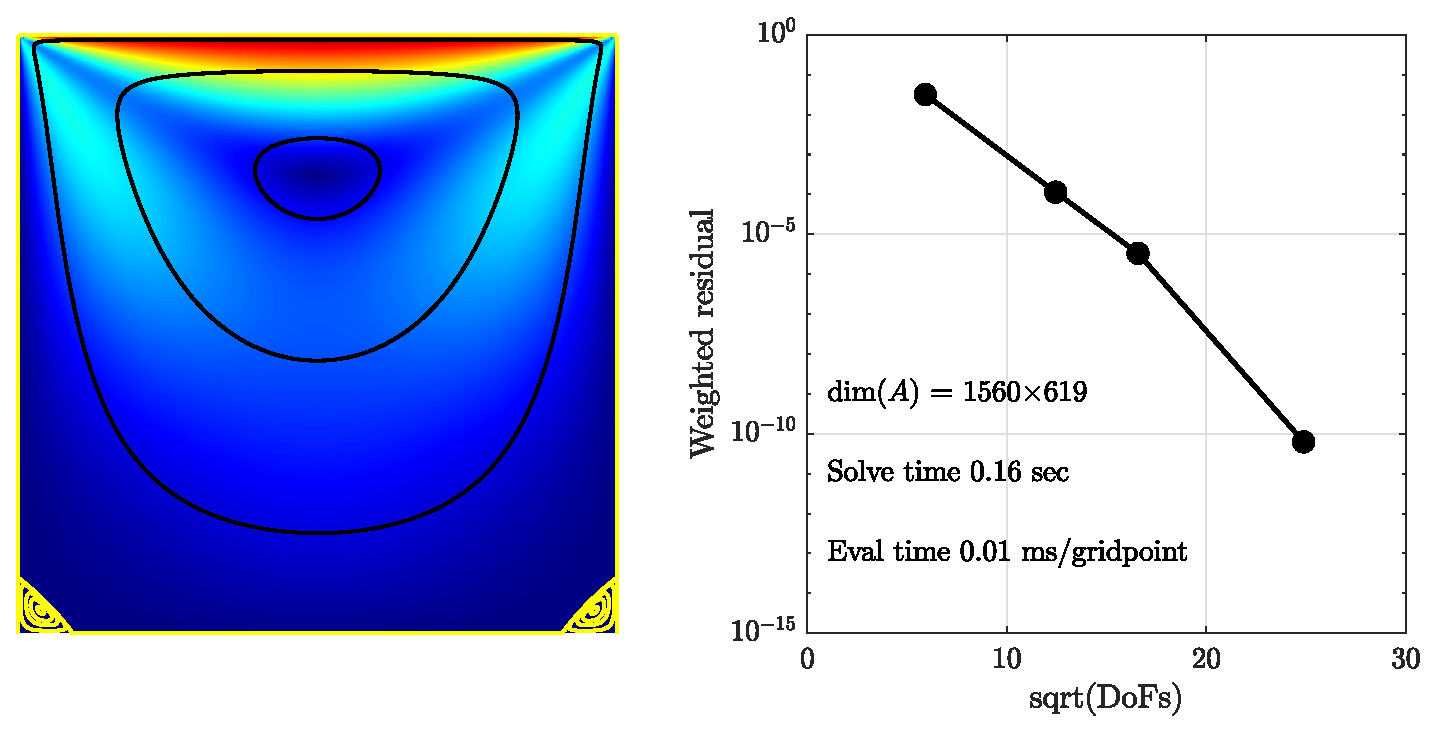
\includegraphics[width=\linewidth]{Figures/ldc}

\vspace{2em}
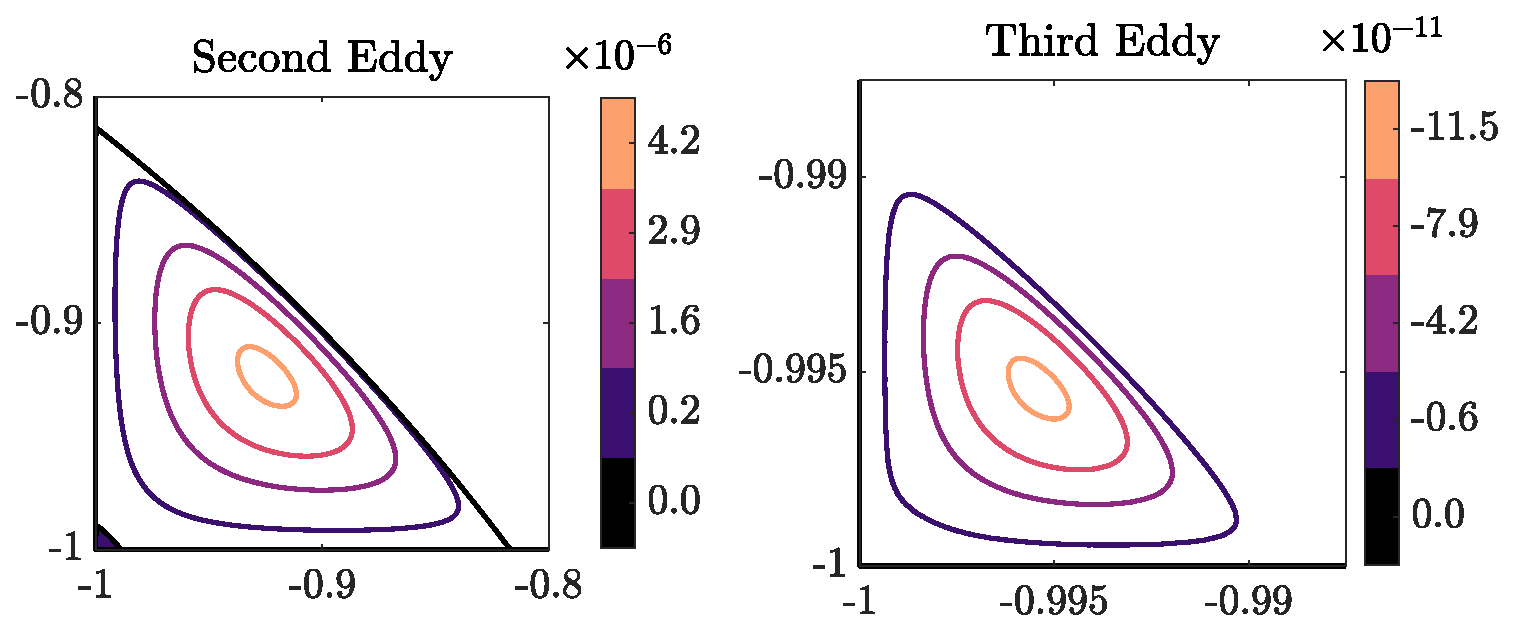
\includegraphics[width=\linewidth]{Figures/ldc_eddy}

\caption{Stokes flow in a square lid-driven cavity solved to 10-digit accuracy
   in 0.14 secs. on a laptop. Stream contours and velocity magnitude (top
   left), convergence (top right), and close-ups of the eddies (bottom).}
\label{fig:ldc}
\end{figure} 
\begin{figure}[H]
\centering
\includegraphics[width=0.9\linewidth]{Figures/ldc_loglog}
\caption{Stream function log-log plot along the $45^\circ$ line for Example
   \ref{ex:square}. The length scale $L=2\sqrt{2}$ corresponds to the diagonal
   of the cavity. The computed solution matches the asymptotic approximation to
   plotting accuracy over an amplitude range of ten orders of magnitude.}
\label{fig:ldc_loglog}
\end{figure}

\end{example}


\begin{example}[Lid-driven triangular cavity.]
\label{ex:triangle}
In terms of boundary conditions and singularities, the situation in Figure
\ref{fig:wedge} is quite similar to the one depicted in the previous
example, except that the bottom wall has now been collapsed into a single
point. Here, the domain is the isosceles triangle with unit leg and vertex
angle $2\alpha = 28.5^\circ$, which corresponds to $\lambda = 9.49 + 4.43i$.
The fact that the corner is sharper than in the previous example introduces
a faster decay rate and a higher frequency in the eddies, since both the
real and imaginary parts of $\lambda$ have been increased. As a consequence,
four eddies can be observed without the need of a close-up.

This particular setup was chosen for direct comparison with experimental images
from Taneda \cite[Fig.~19]{taneda79}, also featured in
\cite[Fig.~10]{vandyke82}, where he used a very similar setup driven by a
rotating cylinder with Reynolds number $1.7\times10^{-1}$. His imagining
technique employed glycerin as the working fluid with suspended aluminum
particles and a photographic exposure time of 90 minutes. Only the first two
eddies were visible from the experiment, as it is extremely difficult to
visualize two Moffat eddies. According to Taneda, ``the reason is that the
relative intensity of successive vortices is the order $10^3$ and therefore
the photographic exposure necessary to visualize two successive vortices is
about $10^3$ times that necessary to visualize a single vortex.''

\begin{figure}[H]
	\centering
	\begin{tikzpicture}
	\usetikzlibrary{calc}
	\node(picA){
	\begin{minipage}{0.45\linewidth}
	\centering
	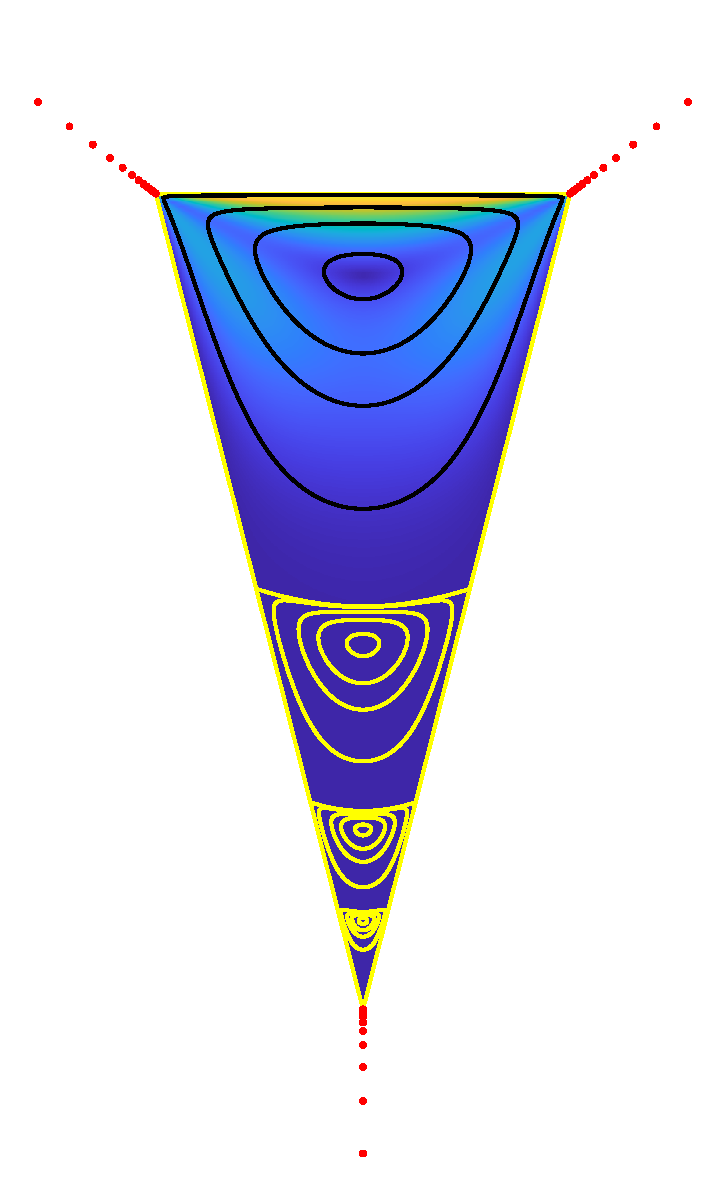
\includegraphics[width=\linewidth]{Figures/wedge}
	\end{minipage}
	\hspace{0.1\linewidth}
	\begin{minipage}{0.45\linewidth}
	\centering
	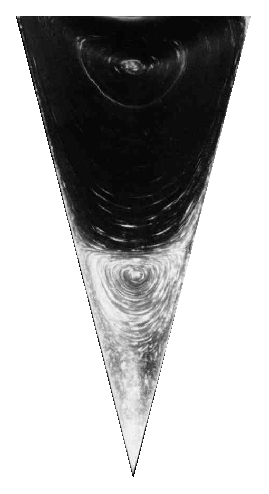
\includegraphics[width=0.6\linewidth]{Figures/wedge_exp}
	\end{minipage}	
	};
	\node at($(picA.south) + (0,3)$){
		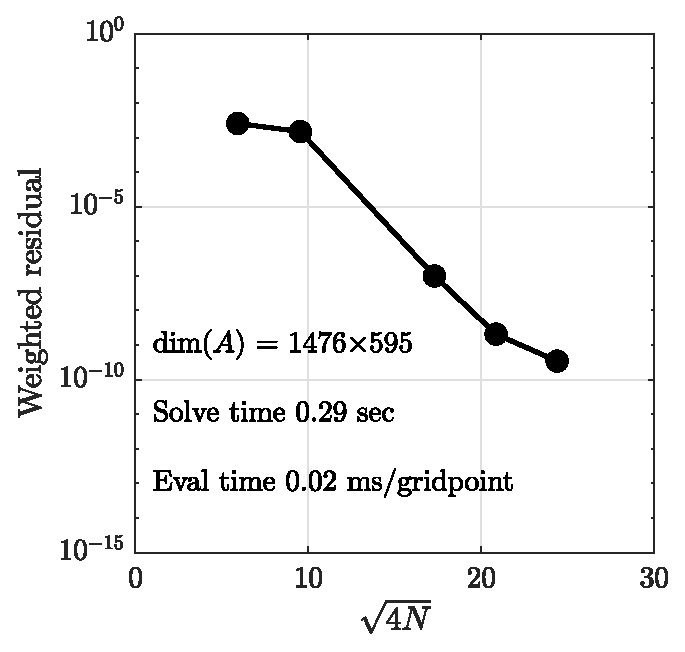
\includegraphics[width=0.4\linewidth]{Figures/wedge_conv}
	};
	\end{tikzpicture}    
	\caption{Stokes flow inside an isosceles triangle of vertex angle $2\alpha=28.5^\circ$.}
	\label{fig:wedge}
\end{figure} 
\begin{figure}[H]
	\centering
	\includegraphics[width=0.9\linewidth]{Figures/wedge_loglog}
   \caption{Stream function log-log plot along the vertical line for Example
   \ref{ex:triangle}. The length scale $L=\cos{\alpha}$ corresponds to the
   height of the triangle. The computed solution matches the asymptotic
   approximation to plotting accuracy over an amplitude range of ten orders of
   magnitude.}
	\label{fig:wedge_loglog}
\end{figure}
\end{example}


\begin{example}[Flow over a step.]
\label{ex:step}
In Figure \ref{fig:step} we have the L-shaped domain $\Omega = [-1,0] \times
[0,1] \cup [0,5]\times[-1,1]$ that resembles a finite section of a pipe with
a sudden expansion or a step. Fully-developed parabolic profiles are imposed
at the inflow and outflow such that mass flow is conserved, i.e.
$(u,v)=(1-(2y-1)^2,0)$ at $x=-1$, $(u,v)=((1-y^2)/2,0)$ at $x=5$, and for
the remaining surfaces we impose a no-slip BC with $\psi_0=2/3$ at $y=1$ and
$\psi_0=0$ on the other walls. We observe more poles clustered near the
re-entrant corner $(0,0)$, where the pressure becomes unbounded. 

This time the main flow is not an eddy, since we have imposed inflow and
outflow BCs. The corner at $(0,-1)$, on which the Moffatt eddies appear,
forms a $90^\circ$ angle as in Example \ref{ex:square}. And once again we
are able to resolve two additional eddies, only that this time the zero
contour on the second eddy can be plotted.

In order to make this example run with lightning speed, it was crucial to
introduce a fake vertex at $(0,1)$. Otherwise, as in the Laplace problem, we
observed that the use of Arnoldi plays a crucial role for convergence.
\begin{figure}[H]
	\centering
	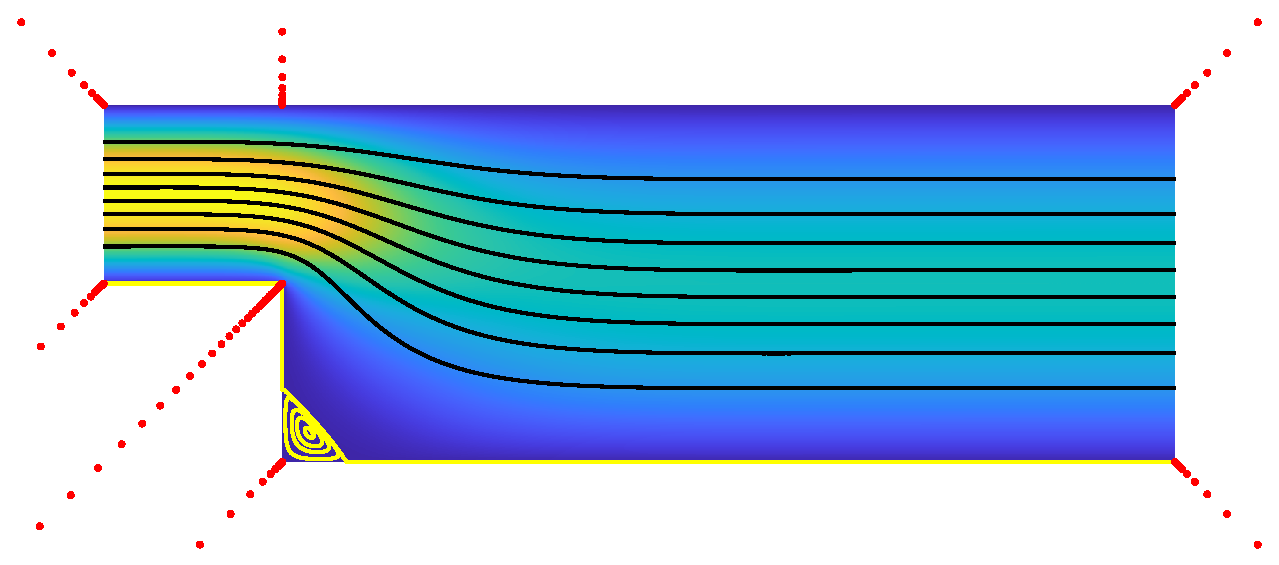
\includegraphics[width=\linewidth]{Figures/step}
	
	\vspace{2em}
	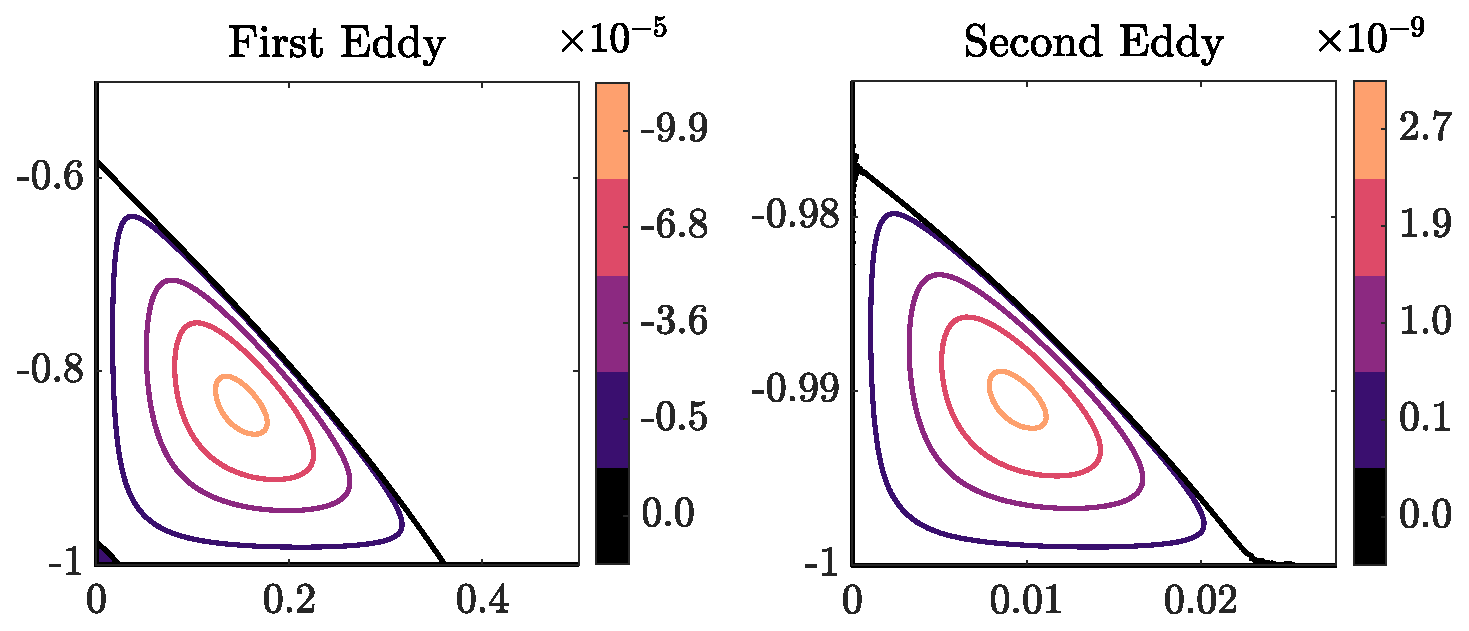
\includegraphics[width=\linewidth]{Figures/step_eddy}
	
	\vspace{2em}
	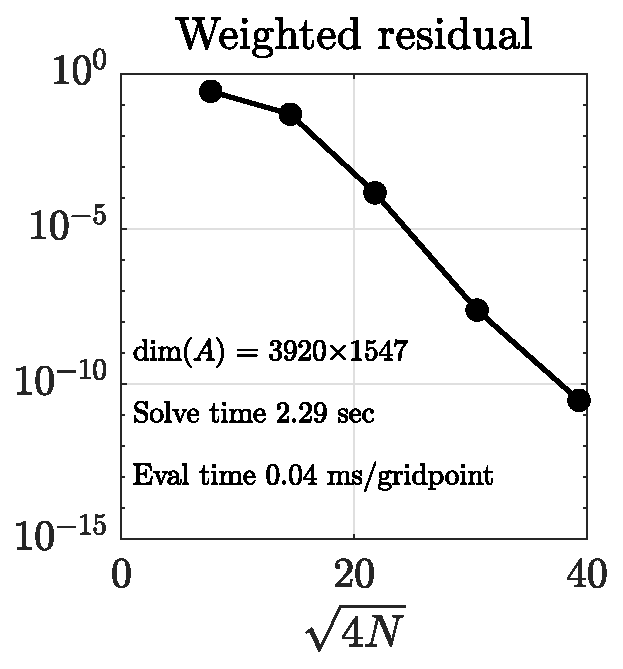
\includegraphics[width=0.4\linewidth]{Figures/step_conv}

	\caption{Stokes flow over a step.}
	\label{fig:step}
\end{figure} 
\end{example}

%------------------------------------------------------------------------------
\section{Unbounded domains \label{sec:unbounded}}
%------------------------------------------------------------------------------

For the unbounded case we rely on the Mobius transformation $w(z)=1/(z-z_0)$
for some $z_0 \in \mathbb{C}\setminus\Omega$, which maps $\infty$ to the origin. By applying the lightning technique on the image of
$\Omega$ under this transformation, we
conclude that we must cluster poles towards infinity in the direction
perpendicular to the channel, and choose sample points along the channel
boundaries that cluster towards infinity.  This is equivalent to inverting the
sign of $\sigma$ in \eqref{eq:poles}.  [TODO: add a figure.]




It is well known that the biharmonic equation is not conformally invariant, in contrast with the Laplace equation. Nevertheless, it was proven by Loewner in \cite{loewner53} that Moebius transformations are indeed the only ones that allow invariance.
\begin{equation}
\hat{\psi} = C \abs{\frac{dw}{dz}}\psi = \abs{w}^2 \psi.
\end{equation} 
Without loss of generality, we set $C=1$ and the 
\begin{equation}
\hat{\nabla}^4\hat{\psi} = 0
\end{equation}
with corresponding boundary conditions
$\hat{\psi}=\hat{h}, \hat{a}\cdot \hat{\nabla}\hat{\psi} = \hat{k}$ on $\Gamma_1$ and $\hat{\nabla}\hat{\psi}=\hat{\vec{g}}$ on $\Gamma_2$. Then, it follows that $\hat{\psi} = \imag{\conj{w}\hat{f}(w) + \hat{g}(w)}$ for some analytic functions $\hat{f}, \hat{g}$.

\begin{equation}
\psi = \abs{z-z_0}^2 \hat{\psi}, \quad u-iv = 2i\frac{\partial \hat{\psi}}{\partial w} + 2i \conj{(z-z_0)} \hat{\psi},
\end{equation}

The example provided in Figure \ref{fig:chan} is the infinite extension of Example \ref{ex:step}.
\begin{figure}[H]
	\centering
	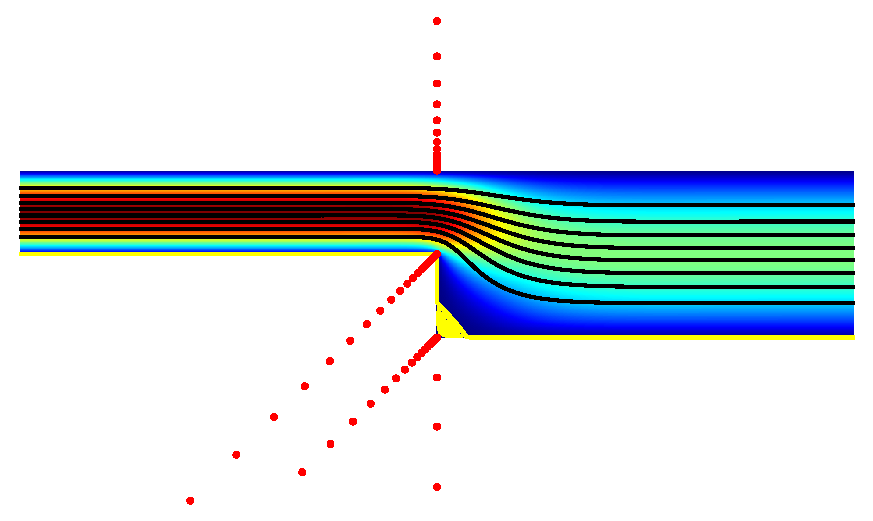
\includegraphics[width=\linewidth]{Figures/chan}
	
	\vspace{2em}
	\begin{minipage}{0.45\linewidth}
		\centering
		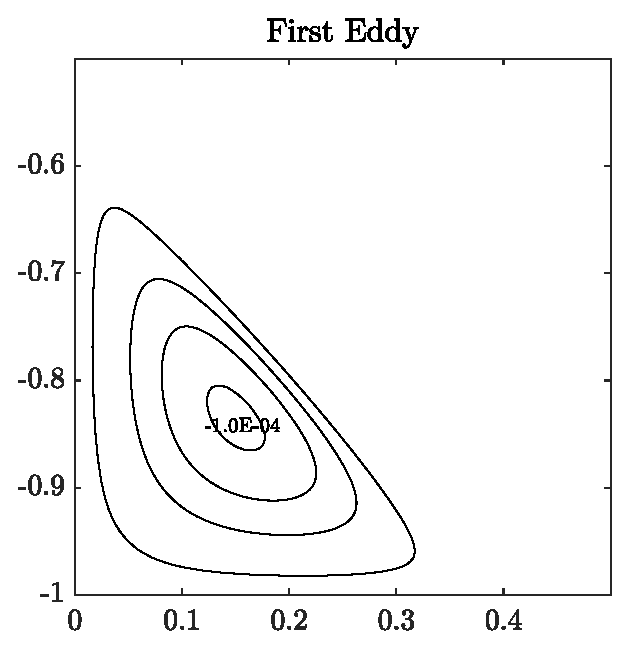
\includegraphics[width=\linewidth]{Figures/chan_eddy}
	\end{minipage}
	\hfill
	\begin{minipage}{0.45\linewidth}
		\centering
		\includegraphics[width=\linewidth]{Figures/chan_conv}
	\end{minipage}
	

	\caption{Stokes flow inside an infinitely long pipe with an expansion.}
	\label{fig:chan}
\end{figure} 


%------------------------------------------------------------------------------
\section{Conclusion \label{sec:conclusion}}
%------------------------------------------------------------------------------




%------------------------------------------------------------------------------
\bibliographystyle{plain}
\bibliography{references}
\end{document}
